\section{Optimizing Histories with Inserts}
\label{sec:optim-reen-hist}

\newcommand{\honlyup}{\history_{noIns}}
\newcommand{\reenactNoR}[1]{\ract{#1 / R}}

In \Cref{sec:dep-ana} and \Cref{sec:up-vc-tb} we have limited the discussion to histories consisting only of update and delete statements. We now introduce an optimization that splits a reenactment query for a history into two parts that can be optimized individually: (i) one part that only simulates update and delete statements over the database at the time of the beginning of the history and (ii) a second part that evaluates the whole history, but only over tuples inserted by insert statements. We use program slicing to optimize (i). The input data size for (ii) is bound by the number of statements in the history and, thus, typically negligible. Note that our symbolic execution technique required by program slicing requires solving a MILP program (an NP-hard problem) whose size is polynomial in the size of the history. Thus, while it may be possible to extend program slicing techniques to deal with inserts, the costs of evaluating (ii) is polynomial in the size of the history and, thus, it is not possible to amortize the cost of program slicing for this part.

We first introduce the idea underlying our optimization, then formally define it, and finally prove its correctness.
Recall from \Cref{def:reenactment-queries} that the reenactment query for an insert statement $\ins{\tup}(R)$ is a union between the state of the relation before the insert and a singleton relation containing the inserted tuple. Updates are reenacted using projections and deletions using selection. As an example consider a history $\history$ consisting of a single insert $u_0$ followed by $n$ update statements $u_1$ to $u_n$. \Cref{fig:insert-opt-before} shows the structure of the reenactment query for this history. Using the standard algebraic equivalences shown below which allow us to pull a union through a projection or selection, we can pull the union up through the projections reenacting the updates of the history. The algebra tree for the resulting query is shown in \Cref{fig:insert-opt-after}. Note that in the rewritten query (i) the right branch only accesses the tuple inserted by the insert statement and (ii) the left input to the union is equal to the reenactment query for a history $\honlyup$ that is the result of deleting the insert statement from $\history$.\\[-6mm]

\begin{align*}
  \projection_A(\query_1  \union \query_2) &\equiv \projection_A(\query_1) \union \projection_{B \to A}(\query_2)\\
  \selection_{\theta}(\query_1 \union \query_2) &\equiv \selection_\theta(\query_1) \union \selection_\theta(\query_2)
\end{align*}

Generalizing this example, the algebraic equivalences shown above are sufficient for rewriting the reenactment query of any history $\history$ without insert statements with queries into a query $\ract{\honlyup} \union \reenactNoR{\history}$ where  $\reenactNoR{\history}$ is derived from $\ract{\history}$ by replacing the subquery (union) corresponding to the first insert $\up$ in the history with the singleton relation $\{t\}$ containing the tuple inserted by $\up$. Importantly, we can apply program slicing to optimize $\honlyup$.


%%%%%%%%%%%%%%%%%%%%%%%%%%%%%%%%%%%%%%%%%%%%%%%%%%%%%%%%%%%%%%%%%%%%%%%%%%%%%%%%
\begin{figure}[t]
  \centering

%%%%%%%%%%%%%%%%%%%%%%%%%%%%%%%%%%%%%%%%
\begin{subfigure}{0.5\linewidth}
  \centering
  \resizebox{0.8\linewidth}{!}{
  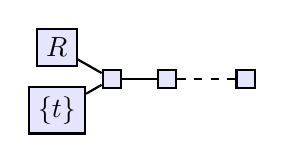
\begin{tikzpicture}
    [
    nod/.style={rectangle,draw=black,fill=blue!10,thick},
    edg/.style={thick},
    ]
    \node[nod] (un) at (2.2,0) {$\projection$};
    \node[nod] (u1) at (1.2,0) {$\projection$};
    \node[nod] (union) at (0.5,0) {$\union$};
    \node[nod] (R) at (-0.2,0.4) {$R$};
    \node[nod] (t) at (-0.2,-0.4) {$\{t\}$};

    \draw[edg,dashed] (un) -- (u1);
    \draw[edg] (u1) -- (union);
    \draw[edg] (union) -- (R);
    \draw[edg] (union) -- (t);
  \end{tikzpicture}
  }
  \caption{Before optimization}\label{fig:insert-opt-before}
\end{subfigure}
%%%%%%%%%%%%%%%%%%%%%%%%%%%%%%%%%%%%%%%%
%%%%%%%%%%%%%%%%%%%%%%%%%%%%%%%%%%%%%%%%
\begin{subfigure}{0.45\linewidth}
  \centering
  \resizebox{0.9\linewidth}{!}{
  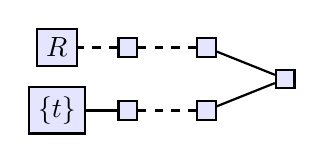
\begin{tikzpicture}
    [
    nod/.style={rectangle,draw=black,fill=blue!10,thick},
    edg/.style={thick},
    ]
    \node[nod] (union) at (2.7,0) {$\union$};

    \node[nod] (lu1) at (1.7,-0.4) {$\projection$};
    \node[nod] (lun) at (0.7,-0.4) {$\projection$};
    \node[nod] (R) at (-0.2,0.4) {$R$};

    \node[nod] (ru1) at (1.7,0.4) {$\projection$};
    \node[nod] (run) at (0.7,0.4) {$\projection$};
    \node[nod] (t) at (-0.2,-0.4) {$\{t\}$};

    \draw[edg] (union) -- (lu1);
    \draw[edg,dashed] (lu1) -- (lun);
    \draw[edg,dashed] (run) -- (R);

    \draw[edg] (union) -- (ru1);
    \draw[edg,dashed] (ru1) -- (run);
    \draw[edg] (lun) -- (t);
  \end{tikzpicture}
  }
  \caption{After optimization}\label{fig:insert-opt-after}
\end{subfigure}
%%%%%%%%%%%%%%%%%%%%%%%%%%%%%%%%%%%%%%%%
\vspace{-3mm}
\label{fig:reenact-opt-example}
  \caption{Structure of an example reeactment query for a history with a single insert. The unions can be pulled up to create two separate queries: the left query accesses R and is the same as the reeactment query for the history without inserts while the right one only accesses inserted tuples.}
\end{figure}



%%% Local Variables:
%%% mode: latex
%%% TeX-master: "historical_whatif"
%%% End:
